\documentclass[singlespace,proposal]{uofsthesis-cs}
\usepackage{graphicx}
\usepackage{amssymb, amsmath}
\usepackage{multirow}
\graphicspath{{/Users/mboots/Documents/2011/beamteam/thesis/data/}}

\usepackage{url}

\renewcommand{\deg}{^\circ }
\newcommand{\dg}{$^\circ$ } 
\newcommand{\dif}{\mathrm{d}} 

% Documentation for the uofsthesis-cs class is given in uofsthesis-cs.dvi
% 
% It is recommended that you read the CGSR thesis preparation
% guidelines before proceeding.
% They can be found at http://www.usask.ca/cgsr/thesis/index.htm

%%%%%%%%%%%%%%%%%%%%%%%%%%%%%%%%%%%%%%%%%%%%%%%%%%%%%%%%%%%%%%%%%%%%%%%%%%%%%%
% FRONTMATTER - In this section, specify information to be used to
% typeset the thesis frontmatter.
%%%%%%%%%%%%%%%%%%%%%%%%%%%%%%%%%%%%%%%%%%%%%%%%%%%%%%%%%%%%%%%%%%%%%%%%%%%%%%

% THESIS TITLE
% Specify the title. Set the capitalization how you want it.
\title{Designing and Optimizing Gratings for Soft X-ray Diffraction Efficiency}

% AUTHOR'S NAME
% Your name goes here.
\author{Mark Boots}

% DEGREE SOUGHT.  
% Use \MSc or \PhD here
\degree{\PhD}         

% EXPECTED CONVOCATION DATE
% Should be month/year, e.g. July 2004
\convocationdate{May 2011}


% NAME OF ACADEMIC UNIT
%
% The following two commands allow you to specify the academic unit you belong to.
% This will appear on the title page as
% ``<academic unit> of <department>''.
% So if you are in the division of biomedical engineering you would need to do:
 \department{Physics and Engineering Physics}
% \academicunit{Division}
%
% The default is ``Department of Computer Science'' if these commands
% are not given.
%
% If you are in a discipline other than Computer Science, uncomment the following line and
% specify your discipline/department.  Default is 'Computer Science'.
% \department{If not Computer Science, put the name of your department here}

% If you are not in a department, but say, a division, uncomment the following line.
% \academicunit{Put the type of academic unit you belong to here, e.g. Division, College}


% PERMISSION TO USE ADDRESS
%
% If you are not in Compuer Science you will want to change the
% address on the Permission to Use page.  This is done using the
% \ptuaddress{}.  Example:
%
 \ptuaddress{Head of the Department of Physics and Engineering Physics\\
 Rm 123 Physics Building\\
 116 Science Place\\
 University of Saskatchewan\\
 Saskatoon, Saskatchewan\\
 Canada\\
 S7N 5E2
 }

% ABSTRACT
\abstract{
For almost two hundred years, diffraction gratings have been -- and still are -- at the heart of many instruments responsible for breakthroughs in scientific understanding.  Today, diffraction gratings are used in astronomy telescopes, chemistry spectrographs, spectrophotometers for life science, and in optics for material science experiments, over a range of wavelengths from the far infrared to soft x-rays.  The sensitivity and speed of these instruments depends on the efficiency of gratings, i.e., the intensity of useful diffracted light compared to the incident light.  In some cases -- such as Peter Zeeman's famous discovery of energy level splitting in a magnetic field -- improvements in grating efficiency make a previously-undetectable effect detectable.  

To support these applications, one component of my graduate work has focussed on the diffraction efficiency of gratings.  While this research happens to be applicable to a wide range of scenarios -- both theoretical and applied, I have been working toward a very tangible application: designing and optimizing an innovative soft x-ray emission spectrometer for the REIXS beamline at the Canadian Light Source.  Over the course of this project, I have created software tools to automate efficiency calculations, used these tools to understand efficiency trends, and applied them to the optical design of the spectrometer.  I have also measured the efficiency of real-world gratings and extensively compared these measurements with calculations.

In this comprehensive report, I present the motivation for this project and some background on both gratings and soft x-ray spectroscopy. I also provide a history of developments in grating theory, explain how we selected the theoretical method I used for modelling grating efficiencies, and introduce this theory.  (For the sake of length constraints, I set up the foundation of the problem, but omit some mathematical details of the algorithms for now.)  In the last chapter, I briefly cover the work that I have already written into my thesis draft, and outline future work to be done.
}

% THESIS ACKNOWLEDGEMENTS -- This can be free-form.
\acknowledgements{
Acknowledgements go here.  Typically you would at least thank your supervisor.
}

% THESIS DEDICATION -- Also free-form.  If you don't want a dedication, comment out the following
% line.
\dedication{This is the thesis dedication (optional)}

% LIST OF ABBREVIATIONS - Sample  
% If you don't want a list of abbreviations, comment the following 4 lines.
%\loa{
%\abbrev{LOF}{List of Figures}
%\abbrev{LOT}{List of Tables}
%}

%%%%%%%%%%%%%%%%%%%%%%%%%%%%%%%%%%%%%%%%%%%%%%%%%%%%%%%%%%%%%%%%
% END OF FRONTMATTER SECTION
%%%%%%%%%%%%%%%%%%%%%%%%%%%%%%%%%%%%%%%%%%%%%%%%%%%%%%%%%%%%%%%%

\begin{document}

% Typeset the title page
\maketitle

% Typeset the frontmatter.  
\frontmatter

%%%%%%%%%%%%%%%%%%%%%%%%%%%%%%%%%%%%%%%%%%%%%%%%%%%%%%%%%%%%%%%%
% FIRST CHAPTER OF THESIS BEGINS HERE
%%%%%%%%%%%%%%%%%%%%%%%%%%%%%%%%%%%%%%%%%%%%%%%%%%%%%%%%%%%%%%%%


% Since thesis chapters are very long and there are a lot of them, it is recommended
% that you put each chapter in a separate .tex file and \input each one of them
% in order.  For example:
%
\input chapter1.tex
\input chapter2.tex

\titlespacing{\chapter}{0pt}{-30pt}{20pt}
\chapter{Current and future work}
\subsubsection{Work currently covered in my thesis draft}
The rest of my thesis draft covers the implementation of this grating theory, and describes the software I wrote to make efficiency calculations more efficient.  Next, I show a comprehensive survey of calculations that can be used by beamline designers to understand trends and factors that affect grating efficiency.  After experimentally validating the calculations, I go on to explain the process I used -- in collaboration with David Muir -- to create an innovative optical design for the REIXS spectrometer.  It turns out that for grating instruments like spectrometers and monochromators, resolution and efficiency are inherently in tension.  By intelligently balancing the trade-offs between these two goals, and exploiting our understanding of efficiency trends and anomalies, we created a design that is predicted to approach world records in both areas (although obviously not simultaneously).  This work was novel because in most cases of beamline design, the grating efficiency is hardly considered, or left to the manufacturer to worry about.

It is even more rare to actually test the gratings for their actual efficiency.  The remainder of my thesis draft describes how I characterized the gratings that were manufactured for our spectrometer, and accounted for differences between the predicted and measured efficiency.  There are very few comparisons of measured and calculated diffraction efficiencies published for the soft x-ray regime; I conjecture that this is because most beamline scientists are so eager upon receiving new gratings to start doing science on their own beamline, that they hesitate to spend time measuring the gratings on another beamline.  In our case, my characterization of the REIXS spectrometer gratings using atomic force microscopy and reflectometer measurements of real-world efficiency turned out to be invaluable: In addition to contributing another set of experimental comparisons, we discovered a substantial manufacturing error in one of the gratings that nearly eliminated its ability to diffract in the useful orders.  We also discovered substantial deviations from the nominal blaze angles of some of the gratings, and adjusted our usage of them accordingly.  Finally, we confirmed the presence of a surface oxide layer on the nickel-coated gratings, and determined how this affects nickel's ideally high reflectivity at soft x-ray wavelengths.  For all of these results, I was able to account for the differences in the real-world gratings using adjusted calculations.

\subsubsection{Future work}
By using a fitting routine to match calculated efficiencies to reflectometer measurements, I have recently discovered that I can use grating efficiency theory to predict the parameters of real-world gratings (such as groove geometry, density, and even non-ideal effects such as surface roughness and oxidation) based on their measured efficiency.  For all of the gratings I studied, the predictions turn out to be consistent with AFM (atomic force microscopy) and PSD (power spectral density) characterization measurements of the actual grating parameters.  This shows that grating efficiency calculations are not only useful in the design and optimization of soft x-ray instruments, but can also be used in the reverse direction as a powerful tool in the characterization of their performance.

Another area of future work focusses on improved numerical implementations of grating theory using massively parallel processing and cloud computing.  All of the rigorous grating methods are computationally expensive, so it can be tedious to calculate efficiency curves over a range of energies, or conduct an optimization of grating parameters. (This is even more true when doing a large number of calculations to attempt to fit a measured efficiency curve.)  The computation can be easily parallelized to take advantage of many processors, but no existing software codes make use of this.  I intend to implement one -- or ideally several -- of the grating theories ``from scratch'' on a grid computing platform; by combining this computing engine with a web-based user interface, it would become possible for beamline designers around the world to benefit from quasi-instant access to grating efficiency results.


% ...
%
% The \input command inserts contents of the specified file at the point of the command.

%%%%%%%%%%%%%%%%%%%%%%%%%%%%%%%%%%%%%%%%%%%%%%%%%%%%%%%%%%%%%%%%
% The Bibliograpy should go here. BEFORE appendices!
%%%%%%%%%%%%%%%%%%%%%%%%%%%%%%%%%%%%%%%%%%%%%%%%%%%%%%%%%%%%%%%%


% Typeset the Bibliography.  The bibliography style used is "plain".
% Optionally, you can specify the bibliography style to use:
% \uofsbibliography[stylename]{yourbibfile}

\uofsbibliography[plain]{thesis_msc_boots.bib}

% If you are not using bibtex, comment the line above and uncomment
% the line below.  
%Follow the line below with a thebibliography environmentand bibitems.  
% Note: use of bibtex is usually the preferred method.

%\uofsbibliographynobibtex


%%%%%%%%%%%%%%%%%%%%%%%%%%%%%%%%%%%%%%%%%%%%%%%%%%%%%%%%%%%%%%%%%%%%%%%%%
% APPENDICES
%
% Any chapters appearing after the \appendix command get numbered with
% capital letters starting with appendix 'A'.
% New chapters from here on will be called 'Appendix A', 'Appendix B'
% as opposed to 'Chapter 1', 'Chapter 2', etc.
%%%%%%%%%%%%%%%%%%%%%%%%%%%%%%%%%%%%%%%%%%%%%%%%%%%%%%%%%%%%%%%%%%%%%%%%%%

% Activate thesis appendix mode.
\uofsappendix

\chapter{Comparison and applicability of\\grating theory families}
\label{methodComparison}
To choose an appropriate grating theory for a particular problem, we need to understand the assumptions and limitations of each method.  As a ``grating method user's guide'', this appendix presents just enough theory to understand the areas of applicability of the integral method, the modal method, and two implementations of the differential method.  This survey is not exhaustive; additional methods have been developed that are only applicable in specific cases.  For example, for certain particular groove profiles, there exist coordinate transformations and ``conformal mappings'', which simplify the boundary conditions so that the grating problem can either be solved analytically, or reduced in complexity.  We concentrate here on the methods that have been intended for general applications.
\section{The Integral Method}
For a perfectly conducting metal, when an electromagnetic is incident on the surface, it will induce a surface current $\mathbf{j}_S(\mathbf{M}')$ at each point $\mathbf{M}'$.  This surface current radiates a field -- the diffracted electric field $E(P)$ at a given point $\mathbf{P}$ above the surface; the field is related to the surface current by the Kirchoff Integral Theorem \cite{Kir83} using the Green's function $G(\mathbf{P}, \mathbf{M}')$:
\begin{eqnarray}
\mathbf{E}(\mathbf{P}) = \int\limits_{\textrm{grating period}} G(\mathbf{P}, \mathbf{M}')\, \phi(\mathbf{M}')\, \dif s'
\end{eqnarray}
where $\dif s$ is a curvilinear coordinate along the grating profile, and $\phi(\mathbf{M'})$ is proportional to the surface current.  Unfortunately, this becomes tricky, because the surface current is not only induced by the incident electric field, but also by the diffracted field radiated from all other points along the grating surface.  This means that the surface current $\mathbf{j}_S(\mathbf{M}')$ at $\mathbf{M}'$ depends not on the incident field, but also on the current $\mathbf{j}_S(\mathbf{M}'')$ at all coordinates $\mathbf{M}''$.  By substituting the corresponding $\phi(\mathbf{M'})$ into the equation above, this transforms it into not a differential equation, but an integral equation for $\phi(\mathbf{M'})$.  

\subsubsection{Limitations}
In practice, the numerical techniques required to solve this integral equation can be complicated, depending on the shape of the profile.  For imperfectly-conducting gratings, the problem becomes even more difficult, and even harder still when the grating is made up of one or many layers -- such as over-coated soft x-ray gratings and multilayers.  Although it is universal, the main limitation of the integral approach is its computational cost, and the programming difficulty of applying it correctly to every unique grating situation; numerical challenges abound, particularly regarding the discretization of the grating profile and how sharp corners and discontinuities are handled.  Reference \cite{Pom91} presents an overview of integral implementations, as well as approximations for reducing the computation time and handling coating layers. The latest version -- referred to as the ``modified integral method'' by Goray, has been the topic of many recent publications \cite{Gor02} \cite {Gor02b} \cite{See02} \cite{Gor05}.

\section{Methods using Maxwell's Equations in differential form}
The remaining two families (the modal method and the differential method) start from Maxwell's equations in differential form.  Within the differential method, there are two variants: the ``classical'' differential method, and the ``Rigorous Coupled Wave'' (RCW) approach.  We present all three here together because they share the same foundation.  They all start by projecting the solution to Maxwell's Equations -- i.e., the strength of the electric or magnetic field of the waves -- onto some periodic basis in the $x$-direction, but with an unknown dependence on $y$.  The task for each method is to determine the $y$-dependence by ensuring the total field satisfies the boundary conditions on the grating surface and at infinite.  The modal method and the RCW method both assume a rectangular groove profile, so that the boundary conditions are simplified: this implies that the tangential and normal field components at the grating interface are purely along either the $x$ or $y$-direction.
\subsection{The modal method}
The modal method assumes a basis of functions that are periodic in $x$, with ``modes'' $F_m$ related to the field $u_m(x)$ as
\begin{eqnarray}
F_m(x,y)=u_m(x) \, \exp \left( i \rho_m y \right)
\end{eqnarray}
where $\rho_m$ is a ``mode constant''.  The total field is assumed to be a linear combination of the modes with unknown amplitudes, and since this field must satisfy the boundary conditions on the surface, it is possible to create a set of linear algebraic equations which can be solved for the mode amplitudes.

\subsubsection{Limitations}
For the modal method, the number of modes and the mode constants $\rho_m$ must be sufficient to fully describe the actual field.  For highly conducting materials, finding appropriate mode constants is difficult, but a technique is available in Ref. \cite{And81}.  

The other obvious limitation of the modal method is to rectangular gratings with vertical groove boundaries.  We can attempt to avoid this limitation by using stacks of thin rectangular gratings to represent an arbitrary shape, as shown in Figure \ref{3a}.  This is called the ``staircase approximation'' for obvious reasons, and is also used in the RCW method.  Unfortunately, no matter how thin the slices are made, this approximation creates sharp edges between the layers at the stair-step corners.  Popov et. al. discovered that for TM-polarized light, this creates unrealistically strong electric fields at the corners, which cannot be physically representative of the true electric field near a smooth grating.  Therefore, algorithms that use the staircase approximation require a larger number of basis components to represent this abruptly changing field, which slows down the computation.  More importantly, even when there are enough components to let the solution converge, the results are not representative of reality. \cite{Pop02} 

\begin{figure}[tbp] %  figure placement: here, top, bottom, or page
   \centering
   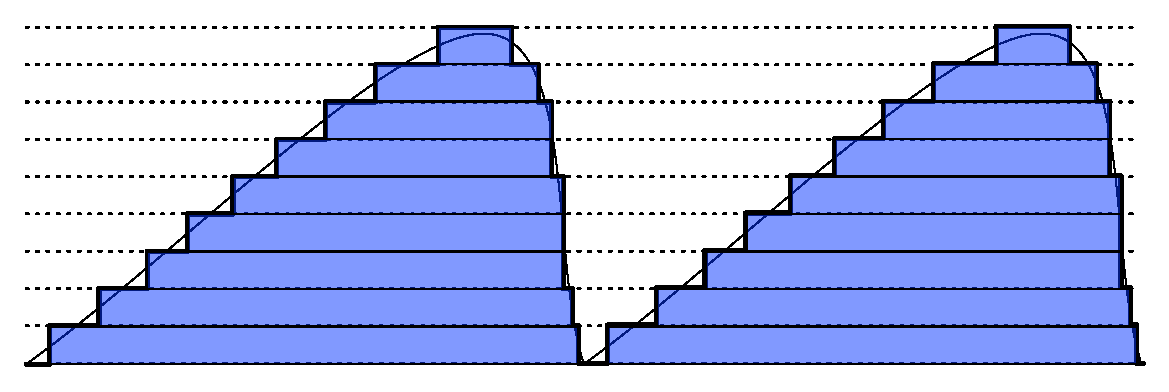
\includegraphics[scale=0.5]{Chapter3/3a_RCWA/3a.pdf} 
   \caption{The modal method and the RCW method approximate every real grating as a stack of rectangular gratings.  This simplifies the boundary conditions (the normal and tangential field components line up either along the $x$- or $y$-axis), so that the problem can be reduced to an algebraic solution for the eigenvalues of the modes or the Fourier coefficients.  Every layer is treated as a separate grating with its own effect on the incoming and outgoing fields; the total grating effect is propagated up the stack using matrix methods.}
   \label{3a}
\end{figure}

\subsection{The differential method}
The differential method's ``classical solution'' uses a periodic field similar to the modal method, except that the basis functions are Fourier terms in the $x$-direction, and the unknown functions to solve are along the $y$-direction:
\begin{eqnarray}
F(x,y)=\exp\left( ik\, \sin \theta_{2}x \right) \sum\limits_m F_m(y) \exp \left( \frac{2\pi i x}{d} \right)
\end{eqnarray}
By matching the total field to the boundary conditions at the top and bottom of the grooves, a set of coupled differential equations is created; this set is solved using a combination of numerical integration and linear algebra, which we describe later in this chapter.  

\subsubsection{Limitations}
The advantage of the classical differential method is that it works for arbitrary groove profiles.  However, for rectangular profiles, it is slower than the other two options because of the necessity to perform a numerical integration for each basis component.  The pure differential method originally suffered from numerical convergence problems in TM polarization on conductive gratings, but these were resolved in 1995 \cite{Li96} \cite{Li96b} \cite{Pop00}.  The only remaining limitation is that the method assumes the material can be described by a well-behaved complex dielectric constant (or the related refractive index) both above and inside the grating material.  This rules out ``perfectly conducting'' (i.e., perfectly reflecting) gratings, for which it is not reasonable to assign a dielectric constant.  This limitation results in a numerical instability when trying to work with nearly perfectly conducting gratings -- for example, gold and aluminum metallic gratings used with deep infrared or millimetre light -- where the real part of the refractive index falls below 0.1.  (A few suggestions have been proposed recently for extending the differential method to highly conducting gratings, such as by substituting a finite-thickness perfectly-conducting layer above an absorbing substrate. \cite{Pop04})

Because this method conducts a numerical integration using assumed starting values along the $y$-direction from the bottom to the top of the grooves, if the grooves are very deep, the long integration distance will increase the computation time.  (Any numerical instabilities associated with the integration will also be increased.)  Therefore, the speed and accuracy of the differential method are reduced for gratings with a very large depth-to-period ratio.\footnote{This limitation is not strictly limited to the differential approach; it will affect the numerical integration of the integral method as well.}

\subsection{The ``Rigorous Coupled Wave'' approach}
The differential method's ``Rigorous Coupled Wave'' approach is a simplification that can be applied for rectangular gratings.  As we mentioned in the case of the modal method, when the groove edges are vertical, the boundary conditions within the grooves are invariant along the $y$-direction.  This means that an eigenvalue technique can be used instead of the full numerical integration along $y$, which reduces the problem to an algebraic solution, speeds up the calculation, and removes the numerical challenges associated with integrating growing exponentials.  As soon as this simplification was proposed, various authors \cite{Bur66} \cite{Pen75} \cite{Moh81} assumed that it could be generalized to arbitrary groove profiles by approximating them with rectangular slices, which could be made as thin as required for a given accuracy; this is the same ``staircase approximation'' used in the modal method.  The RCW approach was used extensively for thirty years, and has been shown to produce fast and accurate results for TE-polarized light on dielectric and absorbing gratings.  However, as we mentioned above, the fundamental validity of the staircase approximation was challenged in Ref. \cite{Pop02}.

\subsubsection{Limitations}
As a differential method, the RCW approach is limited to finitely-conducting materials.  It is also limited to rectangular gratings, or (using the staircase approximation) to stacks of rectangular layers in TE polarization.  It can also produce approximate results in TM polarization for dielectric gratings.

\section{Comparison}
Figure \ref{2e} gives a visual comparison of the limitations and strengths of all four techniques.  It shows that in general there is no clear ``home-run'' universal method; the techniques are complementary rather than supplementary.  The optimal choice for a particular class of grating problems depends on the overlap between the grating characteristics and the limitations of each method.

\begin{figure}[htbp] %  figure placement: here, top, bottom, or page
   \centering
   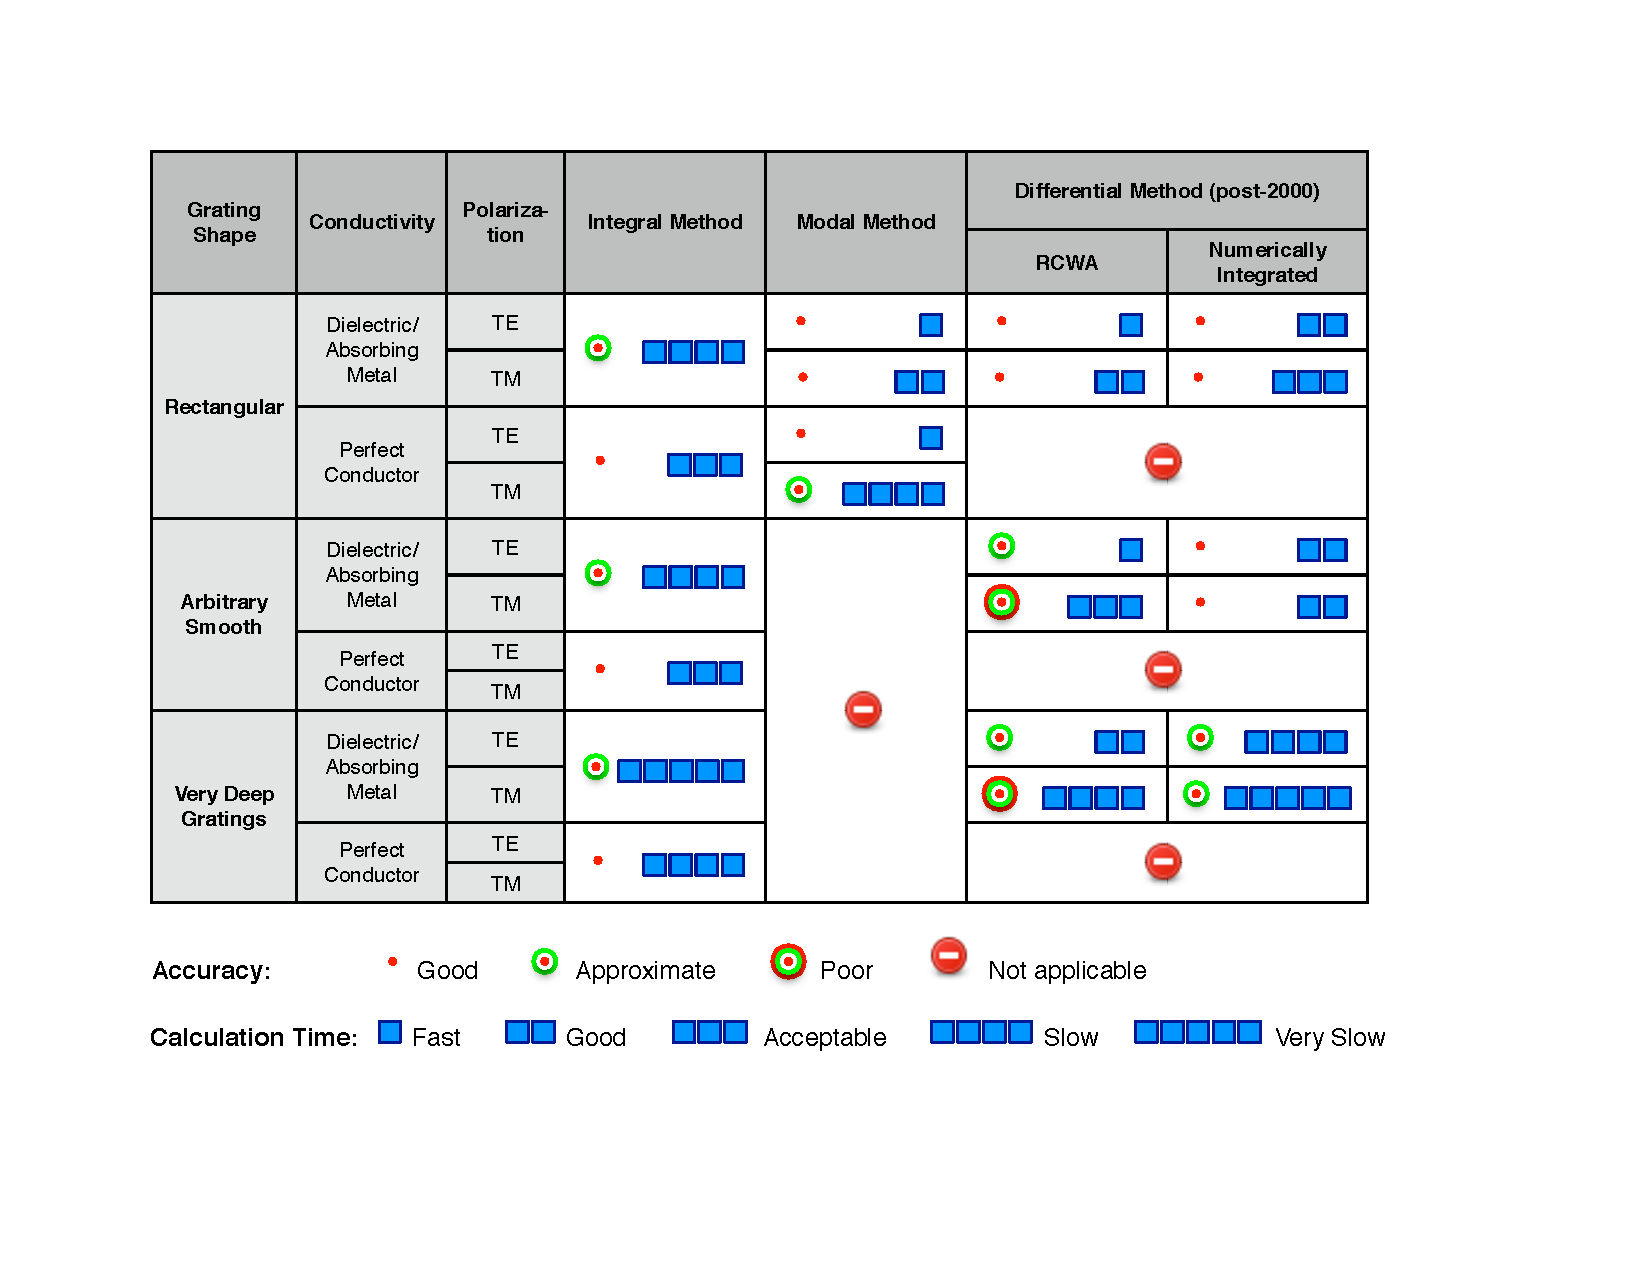
\includegraphics[scale=0.8]{../data/Chapter2/2e_methodComparision/methodComparisonTable_noPre2000.pdf} 
   \caption{A visual comparison of the limitations and strengths of the main methods in grating theory: the integral approach, the modal method, the full (numerically integrated) differential method, and differential method's ``RCW'' staircase-approximation simplification.}
   \label{2e}
\end{figure}

%\chapter{Another Sample Appendix}

%Stuff for this appendix goes here.


\end{document}
